\documentclass[11pt,a4paper,]{article}
\usepackage{lmodern}

\usepackage{amssymb,amsmath}
\usepackage{ifxetex,ifluatex}
\usepackage{fixltx2e} % provides \textsubscript
\ifnum 0\ifxetex 1\fi\ifluatex 1\fi=0 % if pdftex
  \usepackage[T1]{fontenc}
  \usepackage[utf8]{inputenc}
\else % if luatex or xelatex
  \usepackage{unicode-math}
  \defaultfontfeatures{Ligatures=TeX,Scale=MatchLowercase}
\fi
% use upquote if available, for straight quotes in verbatim environments
\IfFileExists{upquote.sty}{\usepackage{upquote}}{}
% use microtype if available
\IfFileExists{microtype.sty}{%
\usepackage[]{microtype}
\UseMicrotypeSet[protrusion]{basicmath} % disable protrusion for tt fonts
}{}
\PassOptionsToPackage{hyphens}{url} % url is loaded by hyperref
\usepackage[unicode=true]{hyperref}
\hypersetup{
            pdftitle={Zomato - Best of Melbourne Analysis},
            pdfborder={0 0 0},
            breaklinks=true}
\urlstyle{same}  % don't use monospace font for urls
\usepackage{geometry}
\geometry{a4paper, centering, text={16cm,24cm}}
\usepackage[style=authoryear-comp,]{biblatex}
\addbibresource{references.bib}
\usepackage{longtable,booktabs}
% Fix footnotes in tables (requires footnote package)
\IfFileExists{footnote.sty}{\usepackage{footnote}\makesavenoteenv{long table}}{}
\usepackage{graphicx,grffile}
\makeatletter
\def\maxwidth{\ifdim\Gin@nat@width>\linewidth\linewidth\else\Gin@nat@width\fi}
\def\maxheight{\ifdim\Gin@nat@height>\textheight\textheight\else\Gin@nat@height\fi}
\makeatother
% Scale images if necessary, so that they will not overflow the page
% margins by default, and it is still possible to overwrite the defaults
% using explicit options in \includegraphics[width, height, ...]{}
\setkeys{Gin}{width=\maxwidth,height=\maxheight,keepaspectratio}
\IfFileExists{parskip.sty}{%
\usepackage{parskip}
}{% else
\setlength{\parindent}{0pt}
\setlength{\parskip}{6pt plus 2pt minus 1pt}
}
\setlength{\emergencystretch}{3em}  % prevent overfull lines
\providecommand{\tightlist}{%
  \setlength{\itemsep}{0pt}\setlength{\parskip}{0pt}}
\setcounter{secnumdepth}{5}

% set default figure placement to htbp
\makeatletter
\def\fps@figure{htbp}
\makeatother


\title{Zomato - Best of Melbourne Analysis}

%% MONASH STUFF

%% CAPTIONS
\RequirePackage{caption}
\DeclareCaptionStyle{italic}[justification=centering]
 {labelfont={bf},textfont={it},labelsep=colon}
\captionsetup[figure]{style=italic,format=hang,singlelinecheck=true}
\captionsetup[table]{style=italic,format=hang,singlelinecheck=true}


%% FONT
\RequirePackage{bera}
\RequirePackage[charter,expert,sfscaled]{mathdesign}
\RequirePackage{fontawesome}

%% HEADERS AND FOOTERS
\RequirePackage{fancyhdr}
\pagestyle{fancy}
\rfoot{\Large\sffamily\raisebox{-0.1cm}{\textbf{\thepage}}}
\makeatletter
\lhead{\textsf{\expandafter{\@title}}}
\makeatother
\rhead{}
\cfoot{}
\setlength{\headheight}{15pt}
\renewcommand{\headrulewidth}{0.4pt}
\renewcommand{\footrulewidth}{0.4pt}
\fancypagestyle{plain}{%
\fancyhf{} % clear all header and footer fields
\fancyfoot[C]{\sffamily\thepage} % except the center
\renewcommand{\headrulewidth}{0pt}
\renewcommand{\footrulewidth}{0pt}}

%% MATHS
\RequirePackage{bm,amsmath}
\allowdisplaybreaks

%% GRAPHICS
\RequirePackage{graphicx}
\setcounter{topnumber}{2}
\setcounter{bottomnumber}{2}
\setcounter{totalnumber}{4}
\renewcommand{\topfraction}{0.85}
\renewcommand{\bottomfraction}{0.85}
\renewcommand{\textfraction}{0.15}
\renewcommand{\floatpagefraction}{0.8}


%\RequirePackage[section]{placeins}

%% SECTION TITLES


%% SECTION TITLES (NEW: Changing sections and subsections color)  
\RequirePackage[compact,sf,bf]{titlesec}
\titleformat*{\section}{\Large\sf\bfseries\color[rgb]{0.8, 0.7, 0.1 }}
\titleformat*{\subsection}{\large\sf\bfseries\color[rgb]{0.8, 0.7, 0.1 }}
\titleformat*{\subsubsection}{\sf\bfseries\color[rgb]{0.8, 0.7, 0.1 }}
\titlespacing{\section}{0pt}{2ex}{.5ex}
\titlespacing{\subsection}{0pt}{1.5ex}{0ex}
\titlespacing{\subsubsection}{0pt}{.5ex}{0ex}


%% TITLE PAGE
\def\Date{\number\day}
\def\Month{\ifcase\month\or
 January\or February\or March\or April\or May\or June\or
 July\or August\or September\or October\or November\or December\fi}
\def\Year{\number\year}

%% LINE AND PAGE BREAKING
\sloppy
\clubpenalty = 10000
\widowpenalty = 10000
\brokenpenalty = 10000
\RequirePackage{microtype}

%% PARAGRAPH BREAKS
\setlength{\parskip}{1.4ex}
\setlength{\parindent}{0em}

%% HYPERLINKS
\RequirePackage{xcolor} % Needed for links
\definecolor{darkblue}{rgb}{0,0,.6}
\RequirePackage{url}

\makeatletter
\@ifpackageloaded{hyperref}{}{\RequirePackage{hyperref}}
\makeatother
\hypersetup{
     citecolor=0 0 0,
     breaklinks=true,
     bookmarksopen=true,
     bookmarksnumbered=true,
     linkcolor=darkblue,
     urlcolor=blue,
     citecolor=darkblue,
     colorlinks=true}

\usepackage[showonlyrefs]{mathtools}
\usepackage[no-weekday]{eukdate}

%% BIBLIOGRAPHY   %------------------------------------------------------------------------------------------------

\makeatletter
\@ifpackageloaded{biblatex}{}{\usepackage[style=authoryear-comp, backend=biber, natbib=true]{biblatex}}
\makeatother
\ExecuteBibliographyOptions{bibencoding=utf8,minnames=1,maxnames=3, maxbibnames=99,dashed=false,terseinits=true,giveninits=true,uniquename=false,uniquelist=false,doi=false, isbn=false,url=true,sortcites=false}

\DeclareFieldFormat{url}{\texttt{\url{#1}}}
\DeclareFieldFormat[article]{pages}{#1}
\DeclareFieldFormat[inproceedings]{pages}{\lowercase{pp.}#1}
\DeclareFieldFormat[incollection]{pages}{\lowercase{pp.}#1}
\DeclareFieldFormat[article]{volume}{\mkbibbold{#1}}
\DeclareFieldFormat[article]{number}{\mkbibparens{#1}}
\DeclareFieldFormat[article]{title}{\MakeCapital{#1}}
\DeclareFieldFormat[article]{url}{}
%\DeclareFieldFormat[book]{url}{}
%\DeclareFieldFormat[inbook]{url}{}
%\DeclareFieldFormat[incollection]{url}{}
%\DeclareFieldFormat[inproceedings]{url}{}
\DeclareFieldFormat[inproceedings]{title}{#1}
\DeclareFieldFormat{shorthandwidth}{#1}
%\DeclareFieldFormat{extrayear}{}
% No dot before number of articles
\usepackage{xpatch}
\xpatchbibmacro{volume+number+eid}{\setunit*{\adddot}}{}{}{}
% Remove In: for an article.
\renewbibmacro{in:}{%
  \ifentrytype{article}{}{%
  \printtext{\bibstring{in}\intitlepunct}}}

\AtEveryBibitem{\clearfield{month}}
\AtEveryCitekey{\clearfield{month}}

\makeatletter
\DeclareDelimFormat[cbx@textcite]{nameyeardelim}{\addspace}
\makeatother

\author{\sf\Large\textbf{ Dea Avega Editya}\\ {\sf\large Master of BA\\[0.5cm]} \sf\Large\textbf{ Muhammad Soban Qasim}\\ {\sf\large Master of BA\\[0.5cm]} \sf\Large\textbf{ Abhishek Sinha}\\ {\sf\large Master of BA\\[0.5cm]} \sf\Large\textbf{ Vinny Vu}\\ {\sf\large Master of BA\\[0.5cm]}}

\date{\sf\Date~\Month~\Year}
\makeatletter
\lfoot{\sf Editya, Qasim, Sinha, Vu: \@date}
\makeatother


%%%% PAGE STYLE FOR FRONT PAGE OF REPORTS    %----------------------------------------------------------------------------------------

\makeatletter
\def\organization#1{\gdef\@organization{#1}}
\def\telephone#1{\gdef\@telephone{#1}}
\def\email#1{\gdef\@email{#1}}
\makeatother
  \organization{ETC5513 Collaborative and Reproductible Practices}

  \def\name{Our consultancy \newline add names \&\newline add names}

  \telephone{(03) 9905 2478}

  \email{questions@company.com}                 %NEW: New email addresss ---------------------------------------

\def\webaddress{\url{http://company.com/stats/consulting/}} %NEW: URl  ------------------------------------------
\def\abn{12 377 614 630}                                    % NEW: ABN -------------------------------------------  
\def\logo{\includegraphics[width=6cm]{logo}}  %NEW: Changing logo
\def\extraspace{\vspace*{1.6cm}}
\makeatletter
\def\contactdetails{\faicon{phone} & \@telephone \\
                    \faicon{envelope} & \@email}
\makeatother

%%%% FRONT PAGE OF REPORTS

\def\reporttype{Report for}

\long\def\front#1#2#3{
\newpage
\begin{singlespacing}
\thispagestyle{empty}
\vspace*{-1.4cm}
\hspace*{-1.4cm}
\hbox to 16cm{
  \hbox to 6.5cm{\vbox to 14cm{\vbox to 25cm{
    \logo
    \vfill
    \parbox{6.3cm}{\raggedright
      \sf\color[rgb]{0, 0.29, 0.55}    % NEW color -company info------------------------------------------------------------------------------------
      {\large\textbf{\name}}\par
      \vspace{.7cm}
      \tabcolsep=0.12cm\sf\small
      \begin{tabular}{@{}ll@{}}\contactdetails
      \end{tabular}
      \vspace*{0.3cm}\par
      ABN: \abn\par
    }
  }\vss}\hss}
  \hspace*{0.2cm}
  \hbox to 1cm{\vbox to 14cm{\rule{4pt}{26.8cm}\vss}\hss\hfill}  %NEW: Thicker vertical line -----------------------------------------------------
  \hbox to 10cm{\vbox to 14cm{\vbox to 25cm{   
      \vspace*{3cm}\sf\raggedright
      \parbox{11cm}{\sf\raggedright\baselineskip=1.2cm
         \fontsize{24.88}{30}\color[rgb]{0, 0.29, 0.55}\sf\textbf{#1}}   % NEW: title color blue ----------------------------------------------
      \par
      \vfill
      \large
      \vbox{\parskip=0.8cm #2}\par
      \vspace*{2cm}\par
      \reporttype\\[0.3cm]
      \hbox{#3}%\\[2cm]\
      \vspace*{1cm}
      {\large\sf\textbf{\Date~\Month~\Year}}
   }\vss}
  }}
\end{singlespacing}
\newpage
}

\makeatletter
\def\titlepage{\front{\expandafter{\@title}}{\@author}{\@organization}}
\makeatother

\usepackage{setspace}
\setstretch{1.5}

%% Any special functions or other packages can be loaded here.
\usepackage{booktabs}
\usepackage{longtable}
\usepackage{array}
\usepackage{multirow}
\usepackage{wrapfig}
\usepackage{float}
\usepackage{colortbl}
\usepackage{pdflscape}
\usepackage{tabu}
\usepackage{threeparttable}
\usepackage{threeparttablex}
\usepackage[normalem]{ulem}
\usepackage{makecell}
\usepackage{xcolor}


\begin{document}           % Begining of document body -----------------------------------------------
\titlepage

{
\setcounter{tocdepth}{2}
\tableofcontents
}
\clearpage

\section*{Introduction}

For this assignment we will be looking at scrapping data from Zomato, one of the largest food aggregators in the world \textcite{zomato}. Zomato provides information on restaurants including, price, location, reviews and more. For the purposes on our analysis we will be looking at the best of Melbourne list \textcite{zomatomelb} to gain insight into some of the most popular restaurants in Melbourne.

This report will include four sections looking at:

\begin{itemize}
\tightlist
\item
  Is expensive food better than cheap food?
\item
  Popularity of different cuisine in Melbourne
\item
  Exploring gluten free food/restaurants in Melbourne
\item
  Distribution of the top 10 restaurants in Melbourne
\end{itemize}

In this report we have used the following packages \textcite{tidyverse}, \textcite{romato}, \textcite{kableExtra}, \textcite{knitr}, \textcite{dplyr}, \textcite{ggplot2}, \textcite{leaflet}, \textcite{rgdal}, \textcite{readr}, \textcite{mapview}, \textcite{viridis}.

\section*{Is expensive food better than cheap food?}

In this section we will be using the Zomato Best of Melbourne to explore whether expensive food is ``better'' than cheap food. To conduct this analysis, we will be looking at:

\begin{itemize}
\tightlist
\item
  What is considered cheap and expensive food
\item
  What the breakdown of price ranges of the restaurants is
\item
  Comparing prices and aggregate ratings
\item
  Determining whether there is a relationship between prices and ratings
\end{itemize}

\hypertarget{what-is-considered-cheap-and-expensive-food}{%
\subsubsection{What is considered cheap and expensive food?}\label{what-is-considered-cheap-and-expensive-food}}

\begin{figure}
\centering
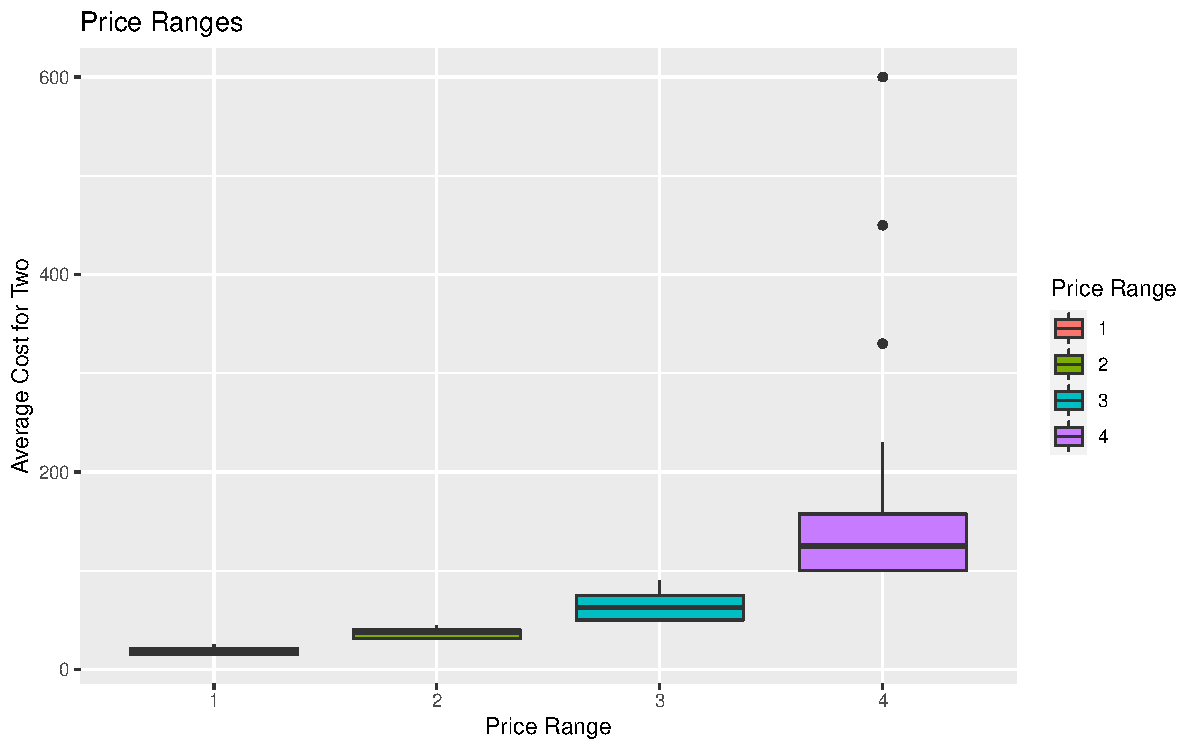
\includegraphics{assignment4_files/figure-latex/price-ranges-1.pdf}
\caption{\label{fig:price-ranges}Price Ranges}
\end{figure}

From Figure \ref{fig:price-ranges} we can see Zomato breaks down price ranges into 4 categories with 4 being the most expensive to 1 being the least expensive.

\begin{table}[!h]

\caption{\label{tab:price-range-table}Price Ranges}
\centering
\begin{tabular}[t]{r|r|r|r|r}
\hline
Price Range & Maximum & Median & Minimum & Range\\
\hline
1 & 25 & 17.5 & 15 & 10\\
\hline
2 & 45 & 37.5 & 30 & 15\\
\hline
3 & 90 & 62.5 & 50 & 40\\
\hline
4 & 600 & 125.0 & 100 & 500\\
\hline
\end{tabular}
\end{table}

From Table \ref{tab:price-range-table} we can see the range of prices that make up each price category.

\hypertarget{what-the-breakdown-of-price-ranges-of-the-restaurants}{%
\subsubsection{What the breakdown of price ranges of the restaurants?}\label{what-the-breakdown-of-price-ranges-of-the-restaurants}}

\begin{figure}
\centering
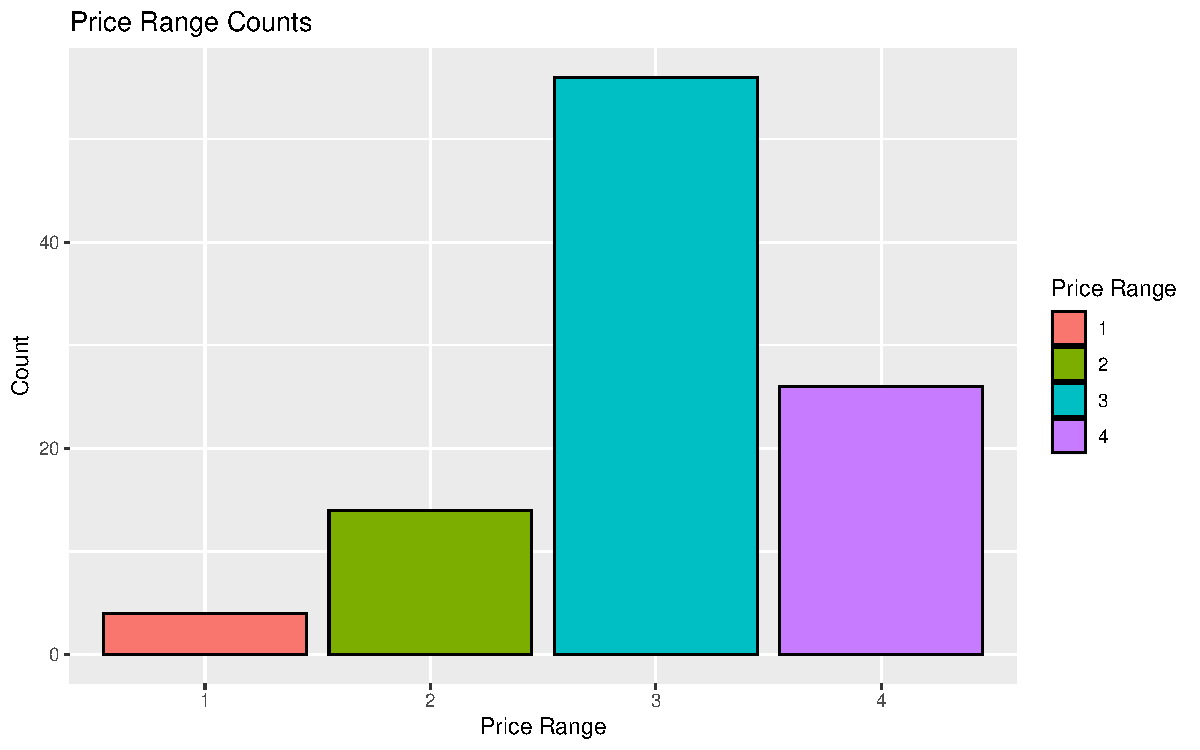
\includegraphics{assignment4_files/figure-latex/price-range-count-1.pdf}
\caption{\label{fig:price-range-count}Price Range Counts}
\end{figure}

From Figure \ref{fig:price-range-count} We can see price range 3 has the most counts. One thing to note however is price range 3 has a range of \$40 compared to 1 and 2 which is \$10 and \$15, respectively. It may be unfair to conclude there is a higher count of more expensive food as the ranges included in the expensive ranges are larger than the lower ones.

\hypertarget{comparing-prices-and-aggregate-ratings}{%
\subsubsection{Comparing prices and aggregate ratings}\label{comparing-prices-and-aggregate-ratings}}

\begin{figure}
\centering
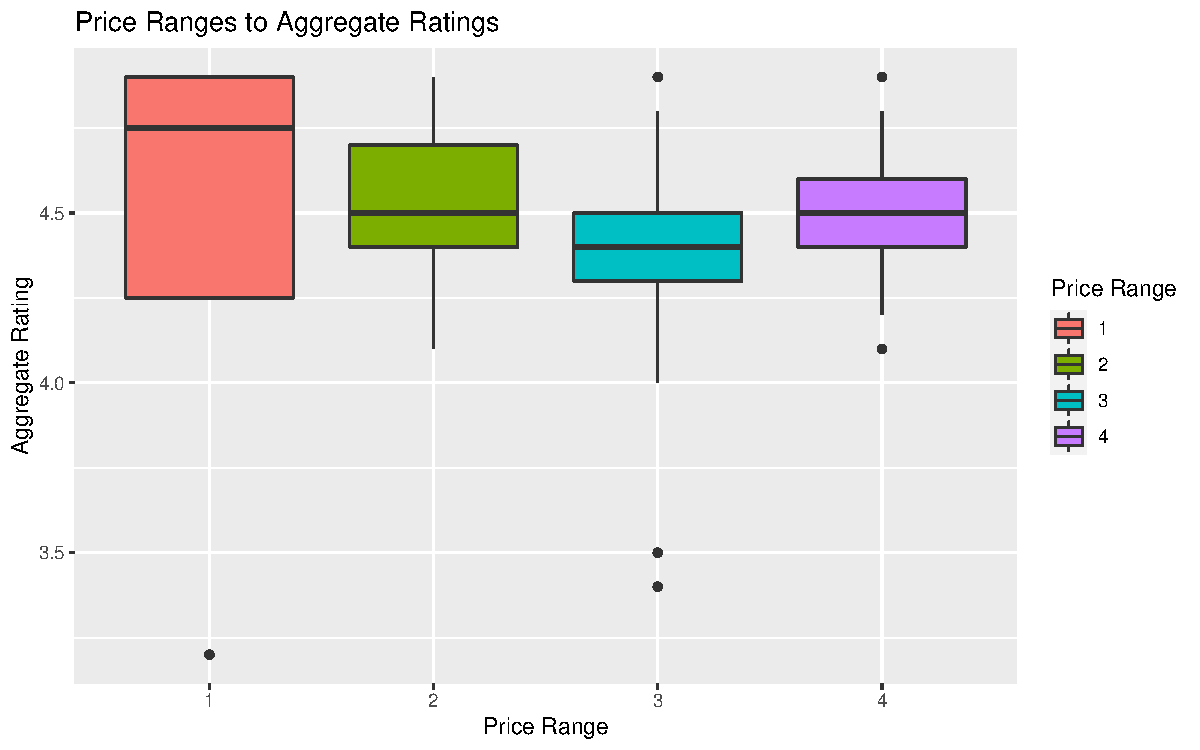
\includegraphics{assignment4_files/figure-latex/price-ratings-1.pdf}
\caption{\label{fig:price-ratings}Price Ranges to Aggregate Ratings}
\end{figure}

From Figure \ref{fig:price-ratings} we can see the median aggregate rating for price range 1 is the highest. In fact, we can see a large amount of lower priced restaurants outranking higher priced restaurants in terms of aggregate ratings.

\hypertarget{is-there-a-relationship-between-prices-and-ratings}{%
\subsubsection{Is there a relationship between prices and ratings}\label{is-there-a-relationship-between-prices-and-ratings}}

\begin{verbatim}
## `geom_smooth()` using method = 'loess' and formula 'y ~ x'
\end{verbatim}

\begin{figure}
\centering
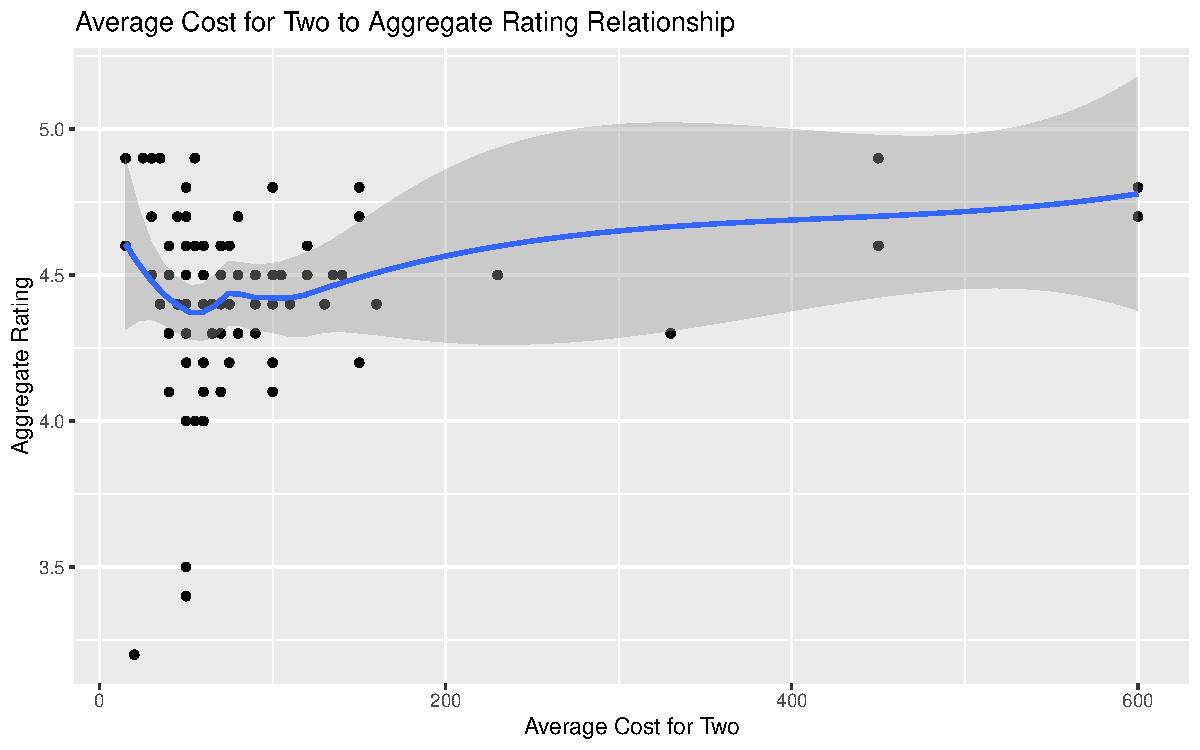
\includegraphics{assignment4_files/figure-latex/cost-rating-relationship-1.pdf}
\caption{\label{fig:cost-rating-relationship}Average Cost for Two to Aggregate Rating Relationship}
\end{figure}

From Figure \ref{fig:cost-rating-relationship} we can see there is not a strong relationship between the average cost for two and the aggregate ratings suggesting there is no relationship between price and food quality. We see a slight upwards trend at the higher price levels. However, this is only based on 5 restaurants with drastically higher prices. We see most of the restaurants fall below the \$200 price point. This might even suggest lower priced restaurants out rank the higher priced restaurants due to the higher count.

\begin{table}[!h]

\caption{\label{tab:rating-ranges}Rating Ranges}
\centering
\begin{tabular}[t]{l|r|r}
\hline
Rating Text & Maximum & Minimum\\
\hline
Average & 3.4 & 3.2\\
\hline
Excellent & 4.9 & 4.5\\
\hline
Good & 3.5 & 3.5\\
\hline
Very Good & 4.4 & 4.0\\
\hline
\end{tabular}
\end{table}

Table \ref{tab:rating-ranges} shows range of aggregate ratings that make up each rating levels.

\begin{figure}
\centering
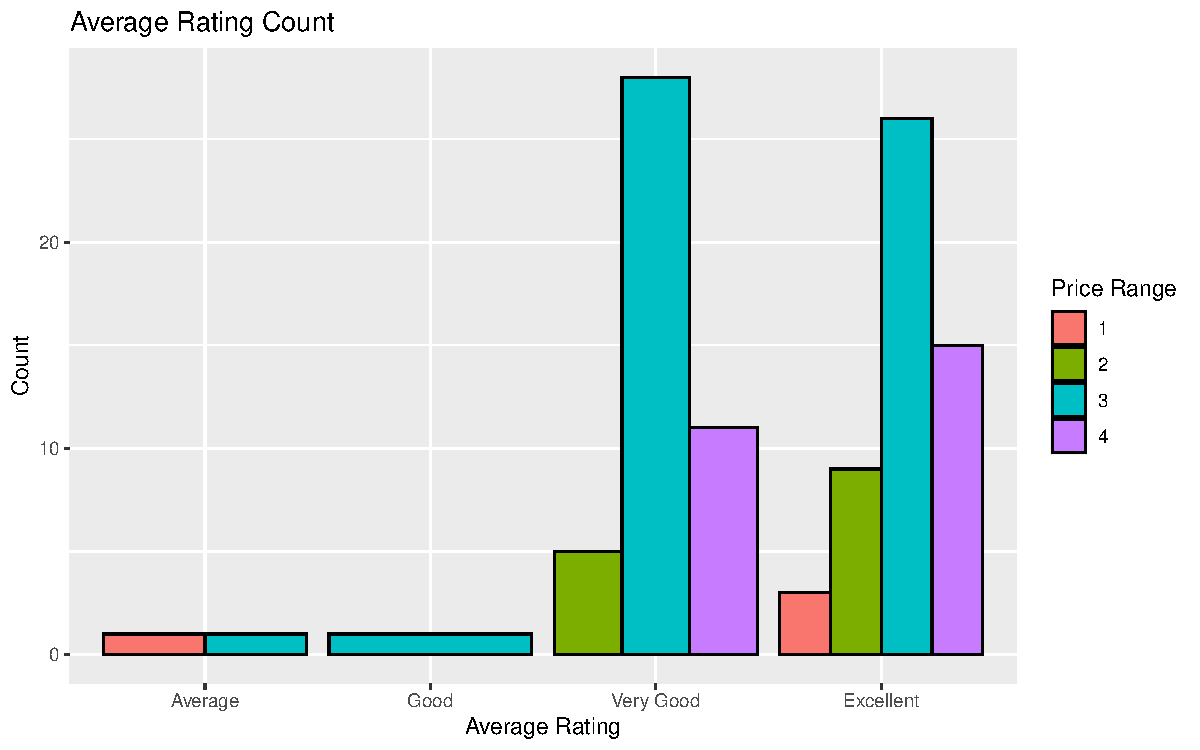
\includegraphics{assignment4_files/figure-latex/rating-count-1.pdf}
\caption{\label{fig:rating-count}Average Rating Count}
\end{figure}

From Figure \ref{fig:rating-count} we can see restaurants in the second and fourth price category all rank in either the very good or excellent category. 3 has the highest count in all categories, however, this may be due to the higher count. We see all price levels have restaurants with high ratings.

\hypertarget{conclusion}{%
\subsubsection{Conclusion}\label{conclusion}}

From this analysis we find there is no real relationship between restaurant prices and quality suggesting expensive food is not better than cheap.

\printbibliography

\end{document}

